\documentclass[a4paper]{article}
\usepackage[a4paper]{geometry}
\usepackage{amsmath}
\usepackage{amssymb}
\usepackage[utf8]{inputenc}
\usepackage{graphicx}
\usepackage{booktabs}
\usepackage[russian]{babel}
\usepackage{flafter}
\usepackage{caption}

\title{Лабораторная работа 2.1.3 \\Определение $\frac{C_p}{C_v}$ по скорости звука в газе}
\date{25 апреля 2017 г.}
\author{Вячеслав Ждановский, студент 611 группы ФРКТ\\
Шамиль Вагабов, студент 611 группы ФРКТ\\
Станислав Токарев, студент 611 группы ФРКТ}
\begin{document}
	\pagenumbering{gobble}
	\maketitle
	\newpage
	\pagenumbering{arabic}
	\paragraph{Цель работы:} 1) измерение частоты коебаний и длины волны при резонансе звуковых колебваний в газе, заполнящем трубу 2) определение показателя адиабаты с помощью уравнения состояния идеального газа
	\paragraph{В работе используются:} звуковой генератор ГЗ; электронный осциллограф ЭО; микрофон; телефон; раздвижная труба; теплоизолированная труба, обогреваемая водой из термостата; баллон со сжатым углекислым газом; газгольдер
	\paragraph{Теоретические сведения:}
	Скорость распространения звуковой волны в газах зависит от показателя адиабаты $\gamma$.\\
	Скорость звука в газах определяется формулой:
	\begin{equation}
 	c=\sqrt{\gamma \frac{RT}{\mu}} \implies \gamma=\frac{\mu}{RT}c^2	
	\end{equation}	
	Звуковая волна, распространяющаяся вдоль трубы, испытывает многократные отражения от торцов. Звуковые колебания в трубе являются наложением всех отражённых волн и, вообще говоря, очень сложны. Картина упрощается, если длина трубы $L$ равна целому числу полуволн, то есть когда
	\begin{equation}
	L=n\frac{\lambda}{2}
	\end{equation}
	Если это условие выполнено, то волна, отраженная от торца трубы, вернувшаяся к её началу и вновь отражённая, совпадает по фазе с падающей. Совпадающие по фазе волны усиливают друг друга $\rightarrow$ амплитуда возрастает $\rightarrow$ наступает резонанс.\\
	При звуковых колбеаниях слои газа, прилегающие к торцам трубам, не испытваются смещения. Узлы смещения повторяются по всей длине трубы через $\lambda/2$. Между узлами находятся максимумы смещения (пучности). \\
	Скорость звука связана с его частотой $f$ и длиной волны $\lambda$ соотношением $c=\lambda f$.\\
	Подбор условий, при которых возникает резонанс, можно производить двумя способами: \\ 
	a) при неизменной частоте $f$ и переменной $L$, тогда для последовательных резонансов $L_{n+k}=n\lambda / 2 + k\lambda / 2$
	б) при неизменной длине $L$ и переменной $f$, тогда для последовательных резонансов:
	\begin{equation}
	L=\frac{\lambda _{k+1}}{2}(n+k)
	\end{equation}
	Получаем:
	\begin{equation}
	f_{k+1}=f_1 + \frac{c}{2L}k
	\end{equation}
	Скорость звука, деленная на $2L$, определяется, таким образом, по угловому коэффициенту графика зависимости частоты от номера резонанса.
	\paragraph{Экспериментальная установка:}
	\begin{figure}[ht!]
		\centering
		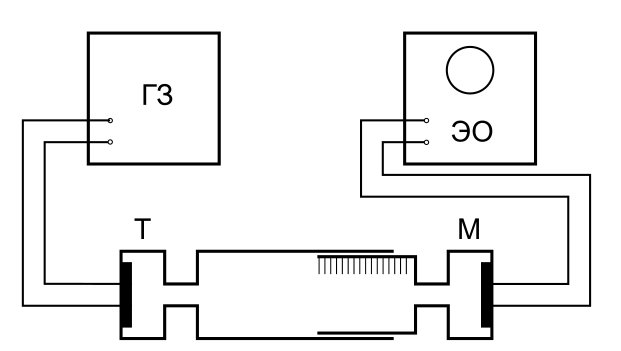
\includegraphics[height=80mm]{pic1.png}
	\end{figure}
	\begin{figure}[ht!]
		\centering
		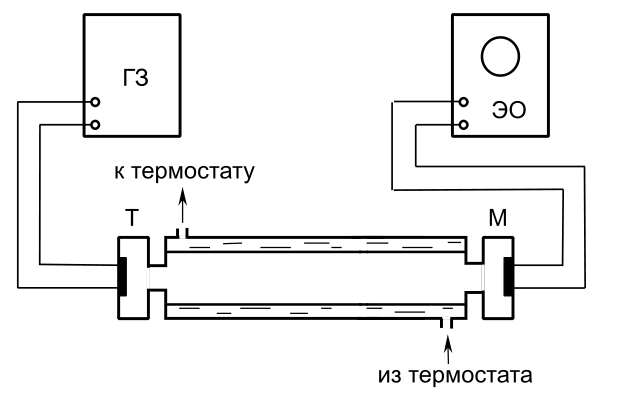
\includegraphics[height=80mm]{pic2.png}
	\end{figure}
	\newpage
	\paragraph{Описание работы установки:}
	Звуковые колебания в трубе возбуждаются телефоном Т и улавливаются микрофоном М. Мембрана телефона приводится в движение переменным током звуковой частоты; в качестве источника переменной ЭДС используется звуковой генератор ГЗ. Возникающий в микрофоне сигнал наблюдается на осциллографе ЭО. \\
	Микрофон и телефон присоединены к установке через тонкие резиновые трубки. Тонкая связь достаточна для возбуждения и обнаружения звуковых колебаний в трубе и в то же время мало возмущает эти колбания: при расчётах оба торца трубы можно считать неподвижными, а влиянием соединительных отверстий пренебречь. 
	\paragraph{Ход работы:}
	$L=(370\pm 5 mm)$ - длина трубы. $p=767$ мм. рт. ст.
	Плавно увеличивая частоту генератора, получим ряд последовательных резонансых значений частоты, отмечая момент резонанса по увелчиению амплитуды колебаний на экране осциллографа.
	\begin{table}[h!]
 		\centering
	\begin{tabular}{|c|c|c|c|c|c|c|}
\hline
		k, номер резонанса & 1 & 2 & 3  & 5 & 6 & 7 \\
		\hline
		f, Hz & 477 & 931 & 1428 & 2315 & 2775 & 3238 \\
		\hline
    	\end{tabular}
  		\caption{Измерения для $t=21\pm 0.2 ^oC$}
	\end{table}
	\begin{table}[h!]
 		\centering
	\begin{tabular}{|c|c|c|c|c|c|c|}
\hline
		k, номер резонанса & 1 & 2 & 3  & 5 & 6 & 7 \\
		\hline
		f, Hz & 482 & 941 & 1440 & 2342 & 2812 & 3827 \\
		\hline
    	\end{tabular}
  		\caption{Измерения для $t=30\pm 0.2 ^oC$}
	\end{table}
	\begin{table}[h!]
 		\centering
	\begin{tabular}{|c|c|c|c|c|c|c|}
\hline
		k, номер резонанса & 1 & 2 & 3  & 4 & 5 & 6 \\
		\hline
		f, Hz & 489 & 958 & 1429 & 1967 & 2380&  2853 \\
		\hline
    	\end{tabular}
  		\caption{Измерения для $t=40\pm 0.2 ^oC$}
	\end{table}
	\begin{table}[h!]
 		\centering
	\begin{tabular}{|c|c|c|c|c|c|}
\hline
		k, номер резонанса & 1 & 2 & 3  & 4 & 5 \\
		\hline
		f, Hz & 499 & 972 & 1451 & 1935 & 2415 \\
		\hline
    	\end{tabular}
  		\caption{Измерения для $t=50\pm 0.2 ^oC$}
	\end{table}
	Построим графики зависимостей $f_{k+1}-f_1$ от $k$.
	\begin{figure}[ht!]
		\centering
		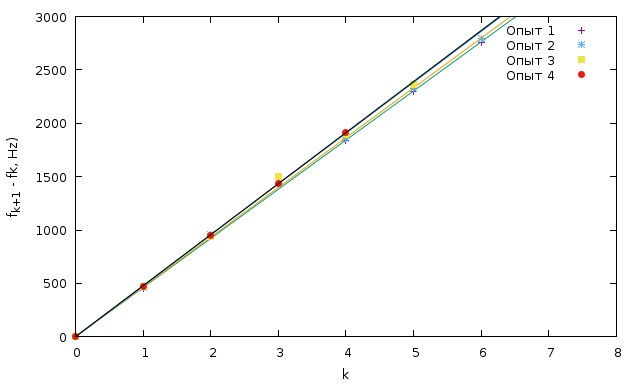
\includegraphics[height=80mm]{plot.png}
	\end{figure}
	Найдем коэффициенты наклона прямых:
	\begin{equation}
	k_1=460.5\pm 3.0 Hz
	\end{equation}
	\begin{equation}
	k_2=466.3\pm 1.6 Hz
	\end{equation}
	\begin{equation}
	k_3=476.7\pm 5.5 Hz
	\end{equation}
	\begin{equation}
	k_4=478.3\pm 0.7 Hz
	\end{equation}
	Отсюда найдем скорости звука и показатели адиабат.
	\begin{table}[h!]
 		\centering
		\begin{tabular}{|c|c|c|c|c|c|}
		\hline
		№ опыта & c, м/c & $\gamma$ \\
		\hline
		1 & $340.8 \pm 5.1$ & $1.38 \pm 0.02$\\
		\hline
		2 & $345.1 \pm 4.8$ & $1.36 \pm 0.03$\\
		\hline
		3 & $352.8 \pm 6.2$ & $1.38 \pm 0.04$\\
		\hline
		3 & $354.0 \pm 4.8$ & $1.36 \pm 0.03$\\
		\hline
		\end{tabular}
  		\caption{Полученные результаты}
	\end{table}
	\paragraph{Подведение итогов:}
	данный метод позволяет получить достаточно точные значения показателя адиабаты.\\
	Большую погрешность в результат эксперминта вносит изменение температуры в помещение, а также возможная негерметичность трубы и примеси в газах.
\end{document}